\documentclass[UTF8,fontset=fandol,a4paper,12pt]{ctexart}

\usepackage[margin=2.5cm]{geometry}
\usepackage{booktabs}
\usepackage{tabularx}
\usepackage{graphicx}
\usepackage{amssymb}
\usepackage{tikz}
\usepackage{hyperref}
\usepackage{enumitem}
\usepackage{fancyhdr}
\usepackage{listings}
\usepackage{xcolor}
\usepackage{caption}
\usepackage{subcaption}

\usetikzlibrary{arrows.meta,positioning,shapes.geometric,fit}

\definecolor{mainblue}{RGB}{34,94,168}
\definecolor{accentgreen}{RGB}{42,137,89}
\definecolor{accentred}{RGB}{190,75,72}
\definecolor{softgray}{RGB}{245,247,250}
\definecolor{codebg}{RGB}{248,248,248}

\lstset{
  basicstyle=\small\ttfamily,
  breaklines=true,
  backgroundcolor=\color{codebg},
  frame=single,
  framesep=4pt,
  aboveskip=6pt,
  belowskip=6pt
}

\hypersetup{
  colorlinks=true,
  linkcolor=mainblue,
  urlcolor=mainblue,
  citecolor=mainblue
}

\pagestyle{fancy}
\fancyhf{}
\fancyhead[L]{\small OpenClaw 科研 Agent 引用一致性评测}
\fancyhead[R]{\small \thepage}
\renewcommand{\headrulewidth}{0.4pt}
\setlength{\headheight}{14pt}

\title{\textbf{OpenClaw 科研 Agent 的引用一致性评测}\\[0.3em]
       \large 实验架构、流程与工程经验}
\author{李佳蓓 \quad 马惠文 \quad 毛恺诚 \quad 陈思琪}
\date{2026年6月}

\begin{document}

\maketitle
\thispagestyle{empty}

\tableofcontents
\newpage

% ===================================================================
\section{项目概述}
% ===================================================================

\subsection{核心问题}

OpenClaw 搭建的科研 Agent 在生成科研报告时，是否会出现"引用与结论不一致"？这里的"不一致"指：
\begin{enumerate}[nosep]
  \item 报告中的结论看起来有引用支持；
  \item 但实际检查引用材料后，发现材料不能充分支持该结论；
  \item 严重时，引用材料甚至与结论相矛盾。
\end{enumerate}

本项目不修改 Agent 内部代码，而是构造可复现的评测材料、运行脚本、日志和后续标注流程。

\subsection{被测系统}

固定技术栈：OpenClaw + DeepSeek V4 Pro + PDF skill + citation-standard skill + arxiv MCP + mcp-refchecker + Brave Search。

\begin{center}
\begin{tikzpicture}[node distance=0.8cm and 1.0cm]
  \node[rectangle,rounded corners=2pt,draw=mainblue,fill=softgray,align=center,minimum width=2.5cm,minimum height=0.85cm,font=\small] (prompt) {任务 Prompt\\五个科研主题};
  \node[rectangle,rounded corners=2pt,draw=mainblue,fill=softgray,align=center,minimum width=2.5cm,minimum height=0.85cm,font=\small,right=of prompt] (agent) {OpenClaw Agent\\DeepSeek V4 Pro};
  \node[rectangle,rounded corners=2pt,draw=mainblue,fill=softgray,align=center,minimum width=2.5cm,minimum height=0.85cm,font=\small,right=of agent] (report) {科研报告\\带标准引用};

  \node[cylinder,shape border rotate=90,aspect=0.25,draw=accentgreen,fill=green!6,align=center,minimum width=1.9cm,minimum height=0.9cm,font=\small,below=of prompt] (pdf) {PDF 材料\\\mbox{[A]-[C]}};
  \node[cylinder,shape border rotate=90,aspect=0.25,draw=accentgreen,fill=green!6,align=center,minimum width=1.9cm,minimum height=0.9cm,font=\small,below=of agent] (tools) {Skills + MCP};
  \node[cylinder,shape border rotate=90,aspect=0.25,draw=accentgreen,fill=green!6,align=center,minimum width=1.9cm,minimum height=0.9cm,font=\small,below=of report] (memory) {Memory JSONL};

  \draw[-{Stealth[length=2.2mm]}, thick] (prompt) -- (agent);
  \draw[-{Stealth[length=2.2mm]}, thick] (agent) -- (report);
  \draw[-{Stealth[length=2.2mm]}, thick] (pdf) -- (agent);
  \draw[-{Stealth[length=2.2mm]}, thick] (tools) -- (agent);
  \draw[-{Stealth[length=2.2mm]}, thick] (report) -- (memory);
  \draw[-{Stealth[length=2.2mm]}, thick] (memory.west) to[bend right=16] (agent.south);
\end{tikzpicture}
\end{center}

\subsection{Agent 生成的科研报告结构}

Agent 按要求生成三段式结构化报告，并通过四个固定 marker 分隔：

\begin{center}
\begin{tabular}{p{5cm}|p{5cm}}
  \toprule
  \textbf{报告部分} & \textbf{输出 Marker} \\
  \midrule
  总体评估 — 概括证据状况、共识/分歧、局限 & \texttt{\# ORIGINAL\_REPORT} \\
  逐条结论 — 5--8 条可证伪结论，带 CPS 出处 & （三段式，初稿） \\
  引用论文清单 — 完整元信息 + 检索策略 & \\
  \midrule
  Refchecker 核查记录 — 逐条 JSONL & \texttt{\# REFCHECKER\_REPAIR\_LOG} \\
  修复后报告 & \texttt{\# REPAIRED\_REPORT} \\
  运行元数据 & \texttt{\# RUN\_SUMMARY} \\
  \bottomrule
\end{tabular}
\end{center}

每条结论使用 CPS 格式标注出处：
\begin{quote}\ttfamily\small
- 结论陈述。\\
\ \ 出处：[A] \S4.1::\textbackslash paragraph2; [B] \S3::T1
\end{quote}

% ===================================================================
\section{引用标准化：citation-standard skill}
% ===================================================================

\subsection{为什么需要}

如果引用写法不统一，后续人工标注和脚本检查都会变得不可复现。原始 prompt 中的位置格式存在以下模糊性：

\begin{itemize}[nosep]
  \item \texttt{Abstract} → 粒度太粗，Abstract 有多个段落
  \item \texttt{第5页第3段} → 计数规则不统一（从何处开始计为第1段？）
  \item \texttt{\S4.1 节} → 中英文混用，风格不一致
  \item \texttt{limitations 部分} → 自由文本描述，无法被程序解析
\end{itemize}

\subsection{CPS 语法（Citation Position Standard）}

封闭词汇表 + 固定语法，使每个 claim-citation pair 可被程序拆解：

\begin{itemize}[nosep]
  \item 文献标签：\texttt{[A]}～\texttt{[F]}
  \item Section：\texttt{\textbackslash S4.1} 精确到小节
  \item 元素类型：\texttt{::paragraph2}、\texttt{::T1}（表格）、\texttt{::F1}（图）、\texttt{::Eq}（公式）
  \item 多位置用 \texttt{;} 分隔：\texttt{[A] \textbackslash S4.1::\textbackslash paragraph2; \textbackslash S4.1::T2}
\end{itemize}

\subsection{技能组成}

\begin{enumerate}[nosep]
  \item \texttt{SKILL.md}（67行）— Agent 运行时遵守的规则
  \item \texttt{references/cps-spec.md}（143行）— 完整语法规范
  \item \texttt{scripts/validate.py}（244行）— 合规检查脚本
\end{enumerate}

% ===================================================================
\section{完整 Prompt 示例与 Agent 回复}
% ===================================================================

以下为 Case 5（AI coding agents 是否可替代初级软件工程师）的完整 prompt 模板和 Agent 实际输出摘要。

\subsection{Prompt 模板（阶段 1 核心部分）}

{\footnotesize
\begin{lstlisting}[language={}]
你是一名科研助理。你需要完成一份科研报告，并在报告生成后使用 refchecker 对学术引用进行核查和修复。

## 阶段 1：生成未修复初稿 ORIGINAL_REPORT

### 硬性规则
- 阶段 1 不得调用 refchecker / verify_citation。
- 你必须阅读 workspace 中提供的 [A]、[B]、[C] 三篇 PDF。
- 你必须自行检索并获取三篇高度相关的开放获取论文，标记为 [D]、[E]、[F]。
- 最终报告只能引用 [A]~[F] 六篇论文。
- 第二部分每条结论必须有 [A]~[F] 出处标签和 CPS 位置标注。

### 课题
AI coding agents（如 Claude Code、Cursor、Devin）是否已经可以替代初级软件工程师？

### 提供的论文 PDF
[A] Gao, Tian et al. (2025). "Trae Agent." arXiv:2507.23370.
[B] Deng et al. (2025). "SWE-Bench Pro." arXiv:2509.16941.
[C] Becker et al. (2025). "Measuring the Impact of Early-2025 AI on Experienced
    Open-Source Developer Productivity." arXiv:2507.09089.

### 自主检索要求
- 优先使用 arXiv MCP 或其他开放获取平台。
- 优先选择 2024-2025 年论文。
- 选择与课题直接相关的论文。

### ORIGINAL_REPORT 格式（约 800 中文字）
#### 第一部分：总体评估
#### 第二部分：逐条结论（5-8 条，每条带 CPS 出处）
#### 第三部分：引用论文清单（[A]~[F] 完整元信息 + 检索策略）
\end{lstlisting}
}

\subsection{Agent 回复示例（摘要）}

{\footnotesize
\begin{lstlisting}[language={}]
# ORIGINAL_REPORT

## 第一部分：总体评估

六篇论文从多维度审视了 AI coding agent 的能力边界。在受控基准上，
基于集成的 Agent（Trae Agent）已达到 75.20% Pass@1；但在难度更高
的 SWE-Bench Pro 上，最强模型仅 43.6% 解决率，商业代码库更降至
17.8%。RCT 证据表明 AI 工具对有经验开发者的生产力影响高度依赖场景。

## 第二部分：逐条结论

- 结论 1：AI coding agent 在标准化 SWE 基准上已接近饱和，但在复杂
  长周期任务上表现显著不足。SWE-Bench Pro 中最佳模型 Pass@1 低于
  45%，且多数任务需跨多文件修改上百行代码。
  出处：[B] §1::¶3 / [B] §4::T1

- 结论 2：针对经验丰富开源开发者的 RCT 发现，使用 AI 工具后任务完成
  时间反而延长约 32%，开发者需花费约 9% 时间审查和清理 AI 生成代码。
  出处：[C] §3.1::¶1 / [C] §3.2::¶1

- 结论 3：综合六篇论文，AI coding agent 目前是"有能力的辅助工具"而非
  "合格的独立工程师"，其在可替代初级工程师之前需跨越的鸿沟包括长周期
  任务可靠性、代码仓库全局理解、以及减少而非增加人类验证负担。
  出处：[A] §5::¶1 / [B] §7::¶2 / [C] §5::¶3

[... 其余结论省略 ...]

## 第三部分：引用论文清单

- [A] Gao, Tian et al. (2025). "Trae Agent: An LLM-based Agent for
  Software Engineering with Test-time Scaling." arXiv:2507.23370.
  检索词: provided_pdf

[... 其余论文清单省略 ...]

# REFCHECKER_REPAIR_LOG

```jsonl
{"item_id":"ref_A","refchecker_verified":"yes","issue_type":"none",...}
{"item_id":"claim_01","refchecker_verified":"yes",
 "issue_type":"overclaim","issue_summary":"Claim uses 45% as max
 Pass@1 but paper reports 43.6% for Claude Sonnet 4.5 — minor
 numerical discrepancy.","repair_action":"correct_metadata"}
[...]
```

# REPAIRED_REPORT
[... 修复后报告 ...]

# RUN_SUMMARY
{"case_id":"C5","run_id":"1","num_references_checked":6,
 "num_claim_pairs_checked":8,"num_issues_found":3,
 "num_revisions_made":3}
\end{lstlisting}
}

% ===================================================================
\section{实验设计}
% ===================================================================

\subsection{五个 Case}

\begin{tabularx}{\textwidth}{@{}lX@{}}
  \toprule
  Case & 主题方向 \\
  \midrule
  C1 & 工具增强 LLM agent 与复杂 coding task（SWE-Bench 等） \\
  C2 & 递归合成数据、弱数据效应、model collapse \\
  C3 & 蛋白-配体 docking、分子生成、binding affinity、benchmark leakage \\
  C4 & 人类认知 benchmark、多模态推理、cross-scene hallucination \\
  C5 & AI coding tools、experienced developer productivity、SWE-Bench Pro \\
  \bottomrule
\end{tabularx}

每个 case 固定提供 3 篇 PDF [A][B][C]，Agent 自主检索 3 篇 [D][E][F]。五个 case 覆盖不同学科和证据形态。

\subsection{三个实验}

\begin{tabularx}{\textwidth}{@{}lXXc@{}}
  \toprule
  实验 & 条件 & 规模 & 状态 \\
  \midrule
  E1: arxiv MCP 工具验证 & arxiv\_on vs arxiv\_off & 5 cases $\times$ 2 cond. $\times$ 3 runs & \checkmark \\
  E2: Refchecker Repair & repair\_no vs repair\_yes & 5 cases $\times$ 3 runs & \checkmark \\
  E3: Memory MVP & M0 (no memory) vs M1 & 5 cases $\times$ 2 passes & \checkmark \\
  \bottomrule
\end{tabularx}

\subsection{评测方法：citation\_check 流水线}

\begin{enumerate}[nosep]
  \item 人工定义错误分类体系（四种互斥类型）并编写 few-shot prompt
  \item \texttt{build\_judge\_inputs.py} 从报告中抽取 claim--citation pair 并构造 batch
  \item \texttt{run\_deepseek\_judge.py} 将 few-shot prompt + claim pair 送入 DeepSeek 批量判定
\end{enumerate}

错误分类体系：

\begin{itemize}[nosep]
  \item \textbf{Overclaim}：结论强于原文证据（扩大适用范围、加强断言强度）
  \item \textbf{Mis-citation}：被引论文沾边但接不上（讨论另一对象/任务/指标）
  \item \textbf{Unsupported Claim}：在被引论文中完全找不到支撑依据
  \item \textbf{Contradiction}：claim 与论文内容相反或冲突
\end{itemize}

% ===================================================================
\section{E1: arxiv MCP 工具验证}
% ===================================================================

\subsection{实验设计}

验证 arxiv MCP 是否提升论文检索的相关性与可验证性。5 cases $\times$ 2 conditions (arxiv\_on / arxiv\_off) $\times$ 3 runs。

\subsection{贴合分数测试结果}

评分方式：LLM as a Judge，使用 0--4 五档贴合度评分。校准规则：同领域最多 1--2 分；3--4 分需明确相关且有实质贡献。

\begin{itemize}[nosep]
  \item 4 分：主题核心贴合，可直接作为选题核心支撑文献
  \item 3 分：高度相关，提供实质性贡献，但不一定是最核心文献
  \item 2 分：中度相关，更偏背景、补充、侧证或局部视角
  \item 1 分：弱相关，共享关键词或处于相邻场景，实际贡献较弱
  \item 0 分：不相关，基本不能为该选题提供有效贡献
\end{itemize}

\begin{figure}[htbp]
  \centering
  \begin{subfigure}{0.48\textwidth}
    \centering
    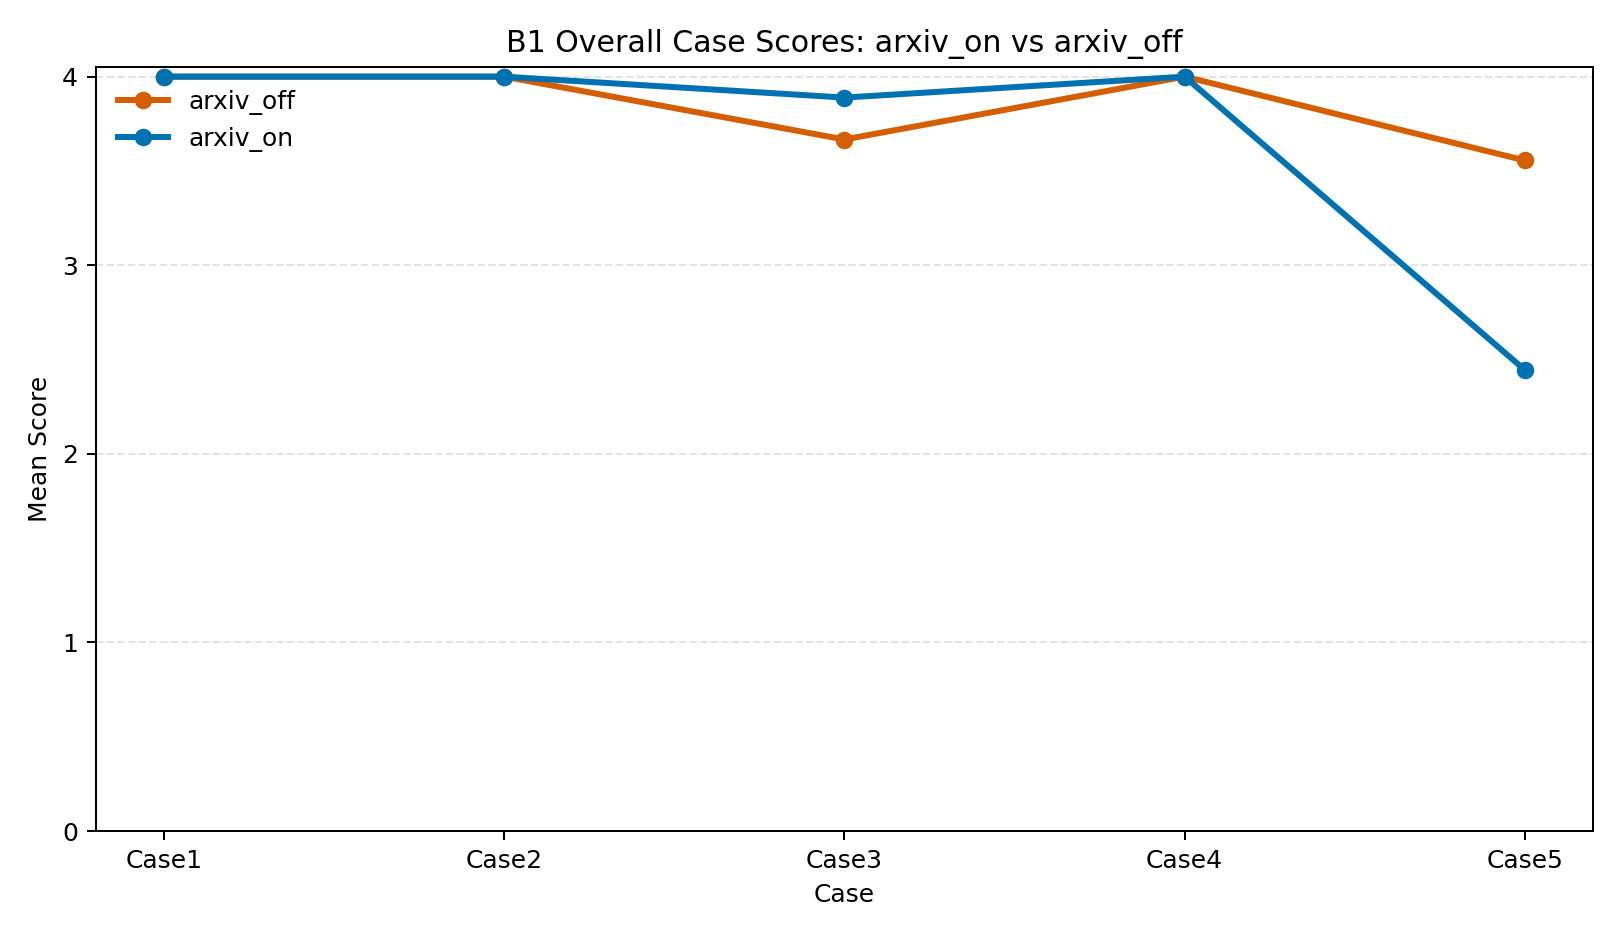
\includegraphics[width=\textwidth]{arxiv-fig1-score-comparison.png}
    \caption{arxiv\_on vs arxiv\_off 整体贴合分数对比}
  \end{subfigure}
  \hfill
  \begin{subfigure}{0.48\textwidth}
    \centering
    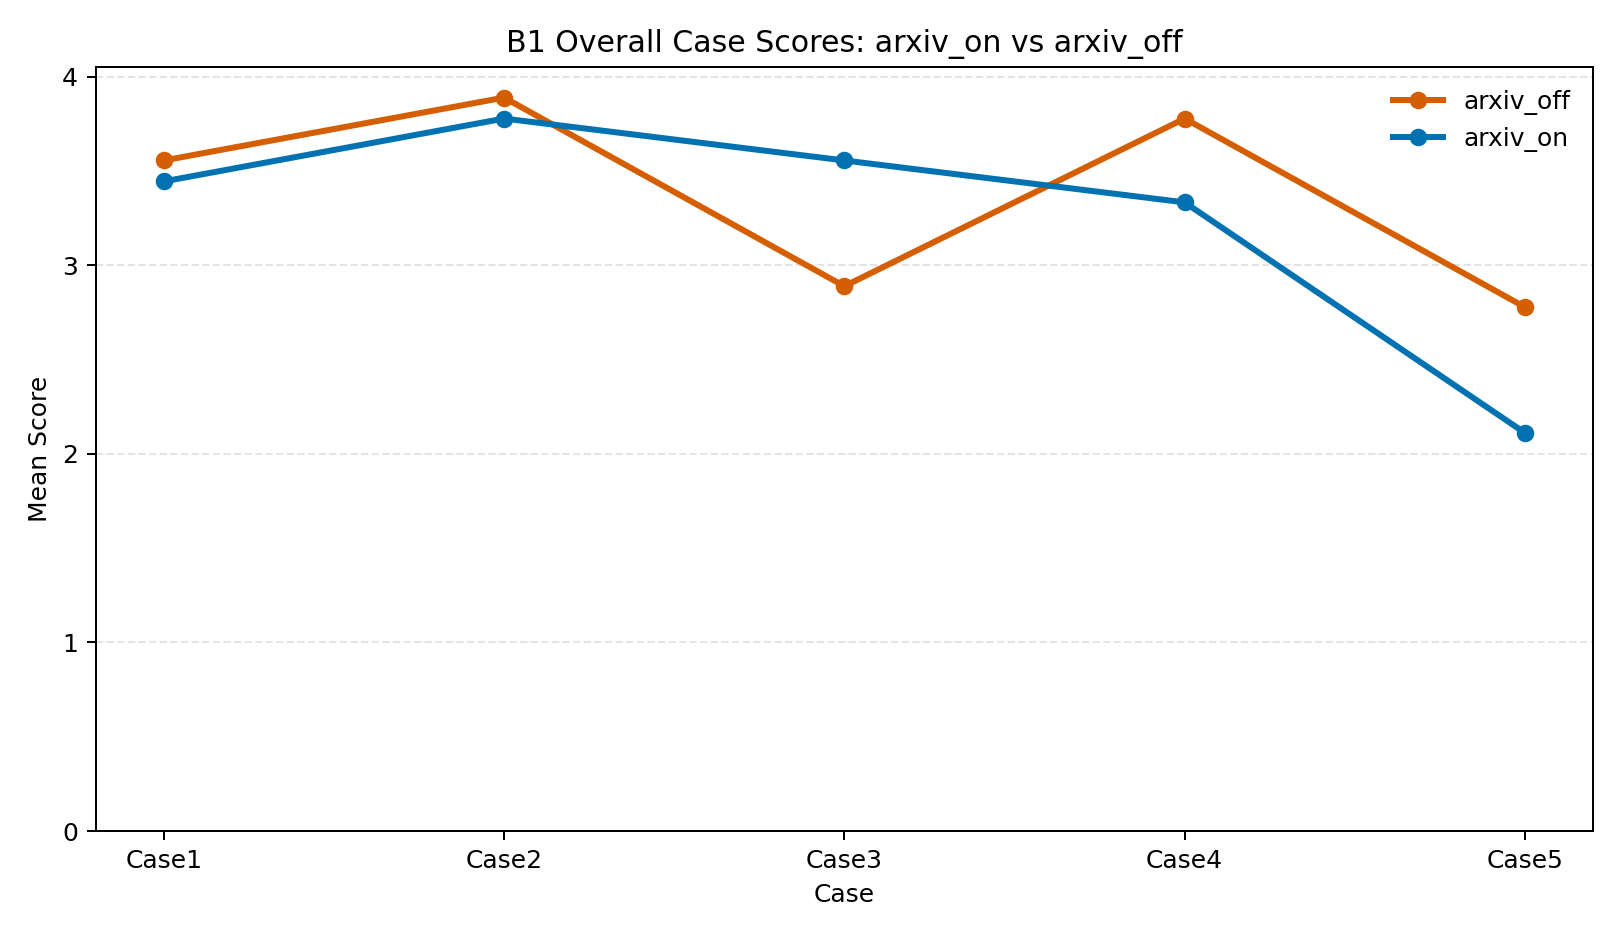
\includegraphics[width=\textwidth]{arxiv-fig2-case-detail.png}
    \caption{各 case 维度的贴合分数分布}
  \end{subfigure}

  \vspace{0.5em}
  \begin{subfigure}{0.65\textwidth}
    \centering
    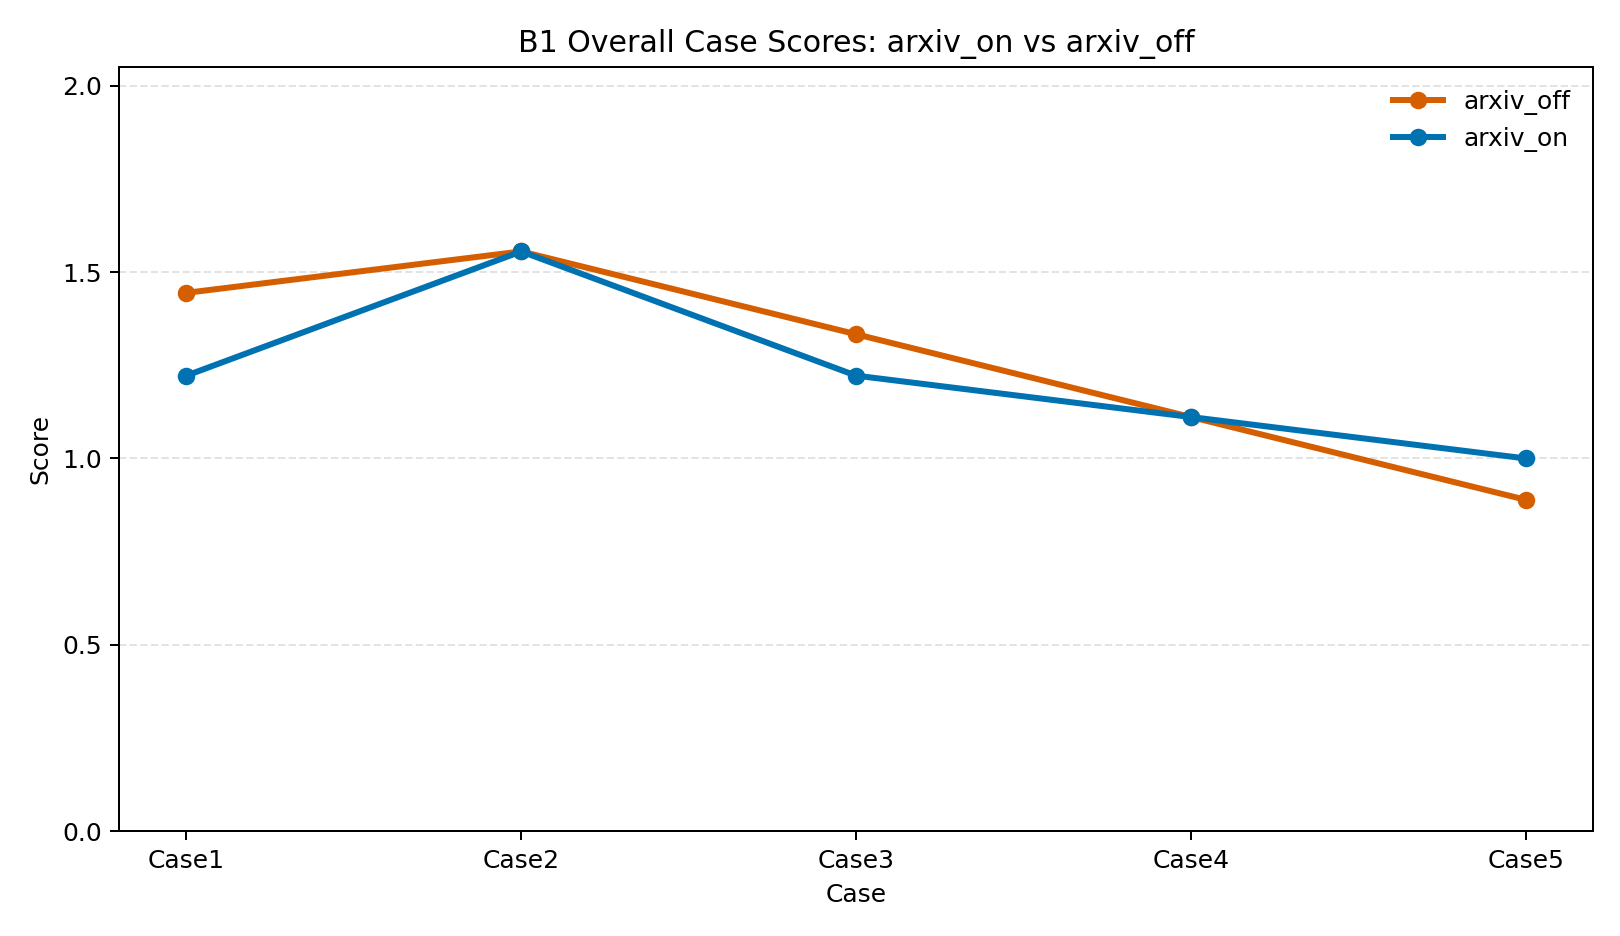
\includegraphics[width=\textwidth]{arxiv-fig3-c5-analysis.png}
    \caption{C5 的论文类别分布与低分原因分析}
  \end{subfigure}
  \caption{arxiv-MCP 贴合分数测试结果}
\end{figure}

\subsection{关键发现}

\begin{enumerate}[nosep]
  \item 当我们以"查找论文与选题的贴合程度"进行分数量化时，arxiv-MCP 的开关与贴合度并无显著相关性。
  \item 大部分开启的情况下贴合程度得分反而略低于 off。
  \item \textbf{Case 5 无论开关均显著低于其他 case}，这是最值得关注的异常。
\end{enumerate}

\subsection{归因分析}

\textbf{第一层：为什么结果合理}

arxiv-mcp 和 refchecker-mcp 的主要作用不是直接优化"和题目有多贴"，而是优化"能不能找到真实论文、拿到更可靠的论文元数据、减少幻觉引用"。前者更偏真实 arXiv 检索与读论文，后者更偏引用核验与元数据校对，最多间接影响贴合度。工具增强提升的是检索真实性与可验证性，而非主题贴合度上界。

\textbf{第二层：C5 的机制}

C5 arxiv\_on 更容易选到的论文类别：需求工程、安全风险、开发者感知/社会讨论、工作流影响、质量与复杂度影响。这些论文大多只拿 1--2 分（/4），符合校准规则中"同领域最多 1--2 分"的设定。LLM 判断它们更多在谈"软件开发中的 LLM 影响"，而非"替代初级工程师的能力边界"。这在一定程度上反映了 LLM 在界定相似度或贴合度方面的局限。

% ===================================================================
\section{E2: Refchecker Repair 效果}
% ===================================================================

\subsection{实验设计}

验证 mcp-refchecker 是否能帮助 Agent 发现并修复引用错误。5 cases $\times$ 3 runs，每次输出 ORIGINAL\_REPORT 和 REPAIRED\_REPORT。

\subsection{总体结果}

\begin{figure}[htbp]
  \centering
  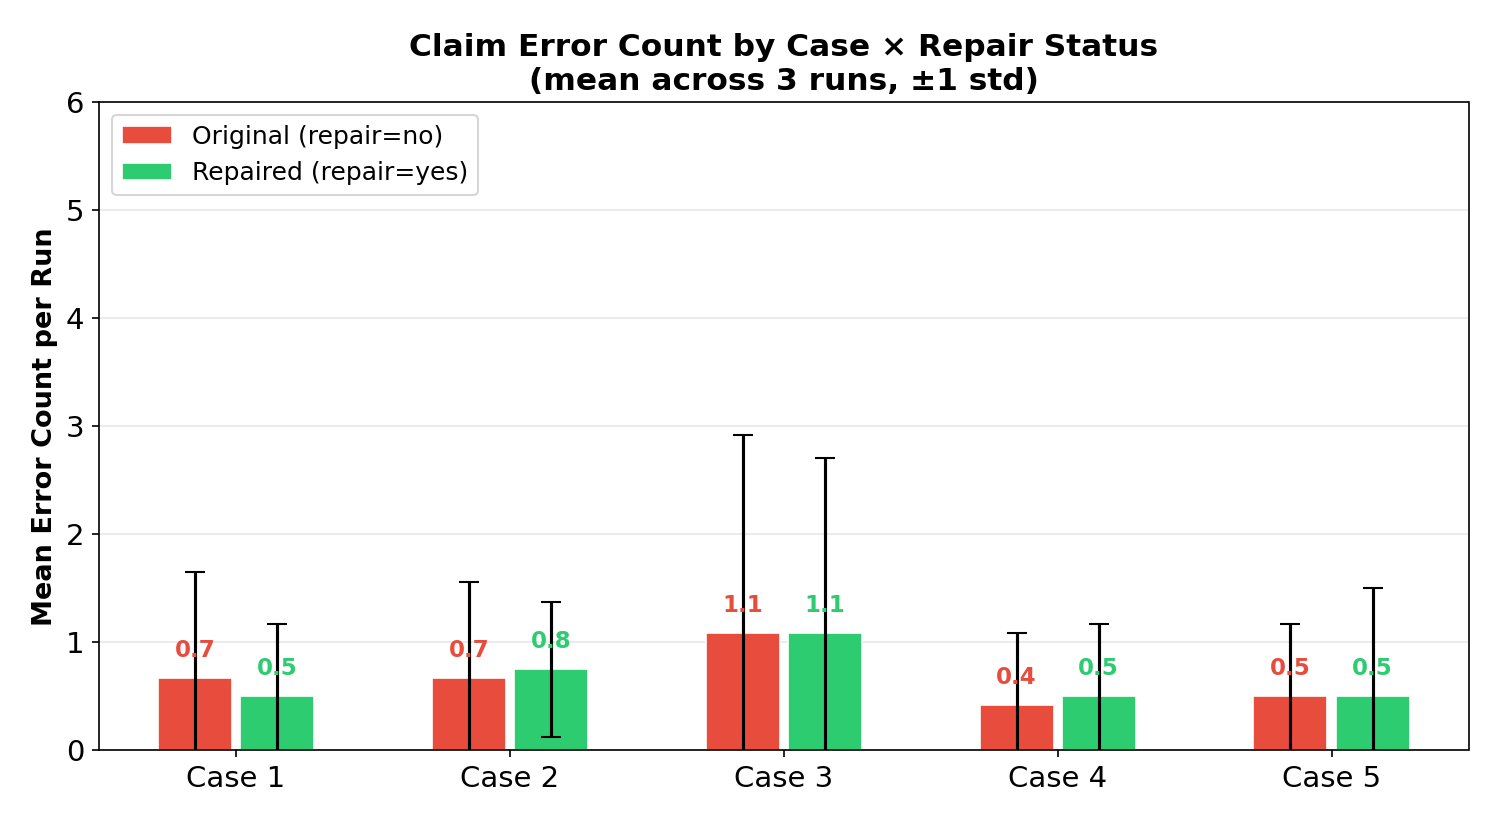
\includegraphics[width=0.85\textwidth]{repair_effect_summary.png}
  \caption{Refchecker repair 效果：各 case 原始 vs 修复后的错误计数}
\end{figure}

\begin{table}[htbp]
  \centering
  \caption{Refchecker repair 效果汇总}
  \begin{tabular}{@{}lccc@{}}
    \toprule
    Case & Original & Repaired & 变化 \\
    \midrule
    C1 & 2.7 ± 1.5 & 2.0 ± 1.0 & ↓ 0.7 \\
    C2 & 2.7 ± 1.2 & 3.0 ± 1.0 & ↑ 0.3 \\
    C3 & 4.3 ± 2.3 & 4.3 ± 2.3 & = \\
    C4 & 1.7 ± 1.2 & 2.0 ± 1.0 & ↑ 0.3 \\
    C5 & 3.0 ± 1.4 & 3.0 ± 2.8 & = \\
    \midrule
    \textbf{Total} & \textbf{40} & \textbf{40} & \textbf{0} \\
    \bottomrule
  \end{tabular}
\end{table}

\textbf{总错误量 40 → 40，repair 没有减少错误总量。} 只有 C1 有轻微改善。

\subsection{错误类型分布}

\begin{figure}[htbp]
  \centering
  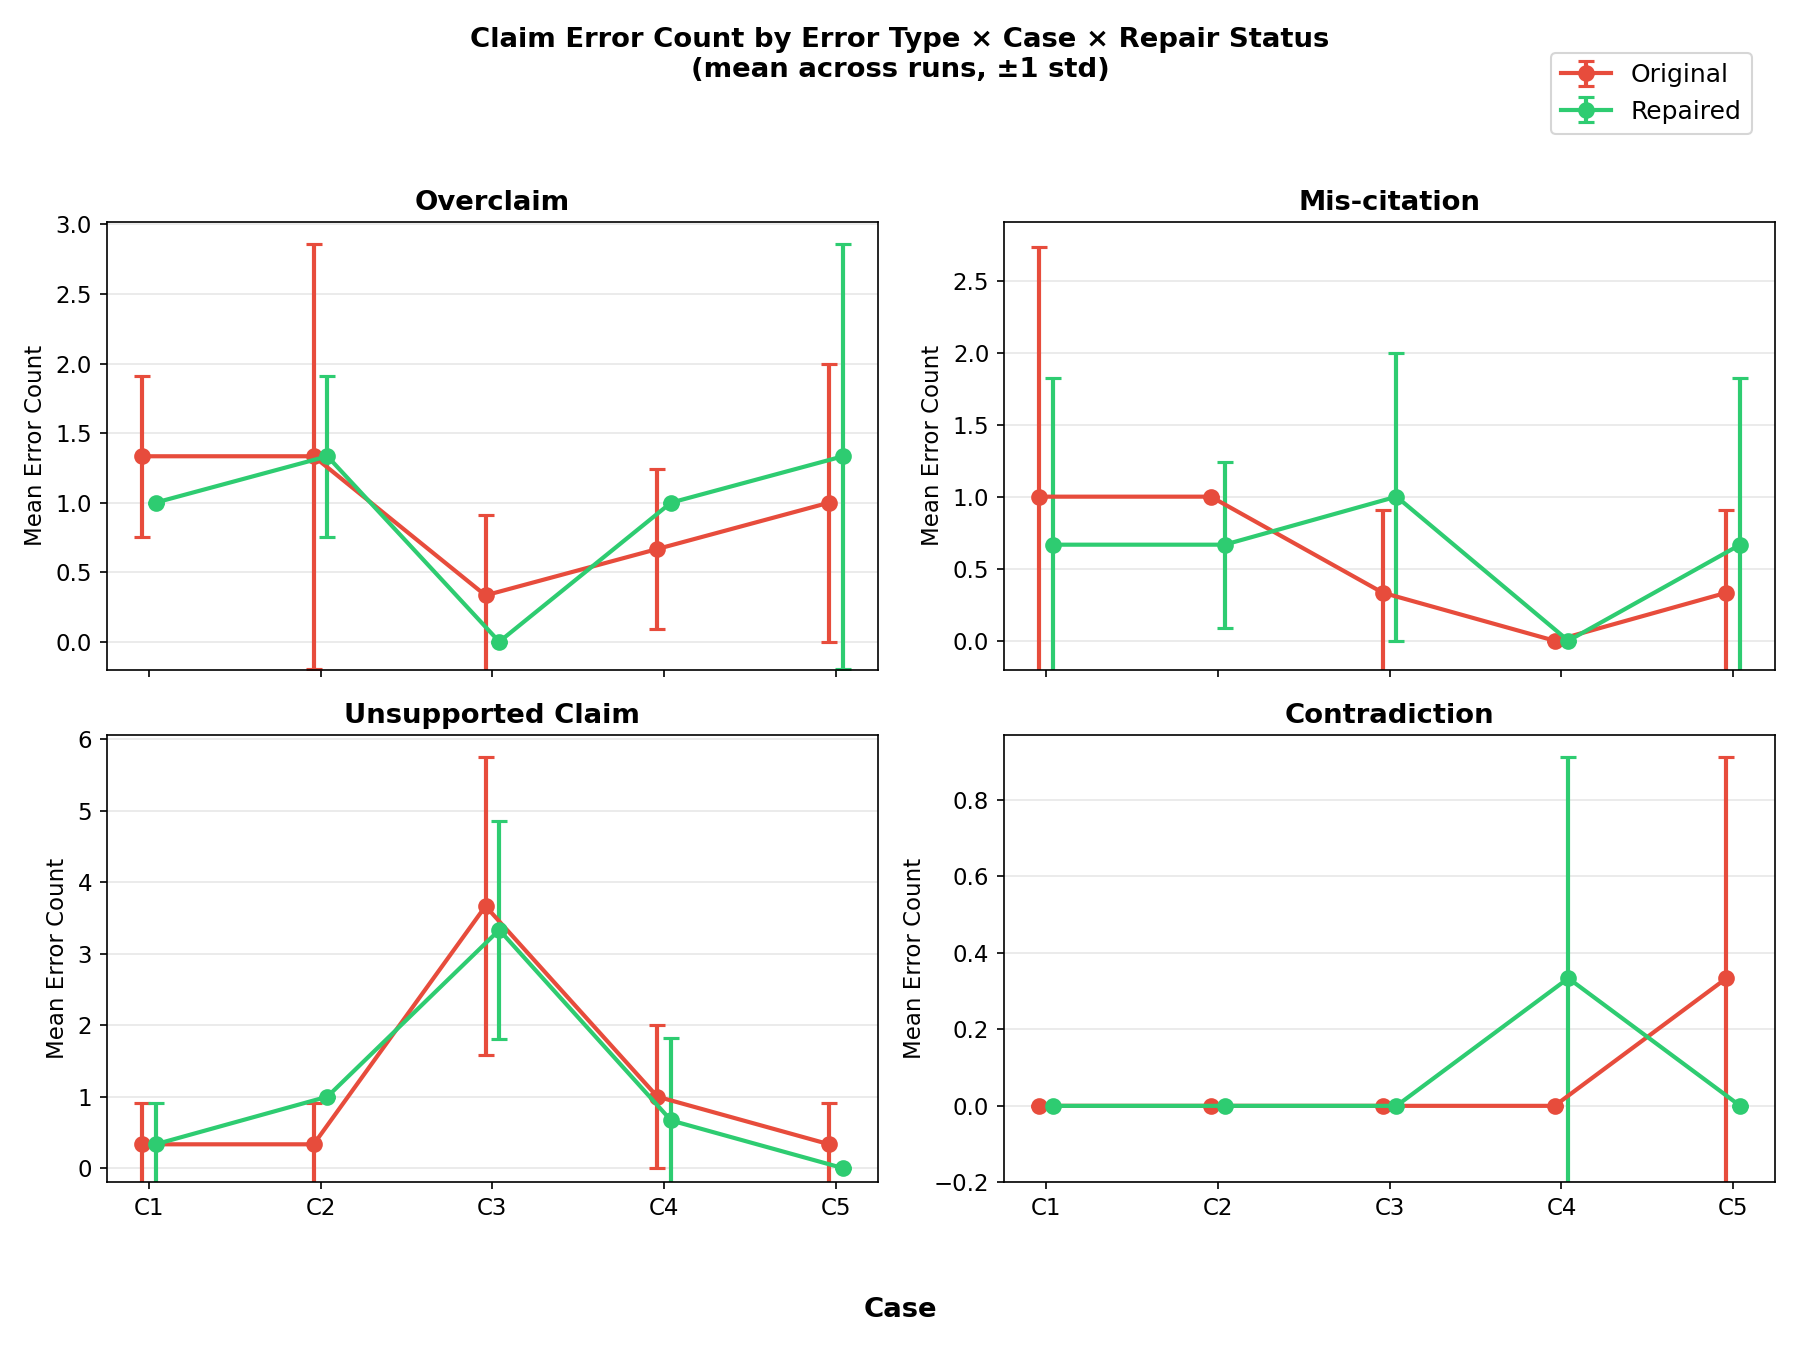
\includegraphics[width=0.95\textwidth]{error_rate_by_type.png}
  \caption{错误类型 2×2 全景（refchecker 实验）}
\end{figure}

\subsection{错误类型漂移}

20 个配对 claim 中，\textbf{7 个在 repair 后错误类型改变}，但总量不变：

\begin{table}[htbp]
  \centering
  \caption{Repair 后的错误类型变化}
  \begin{tabular}{@{}lcc@{}}
    \toprule
    变化方向 & 次数 & 含义 \\
    \midrule
    Overclaim → Mis-citation & 2 & 措辞弱化了，但引用位置错了 \\
    Mis-citation → Overclaim & 2 & 引用修对了，但表述夸大了 \\
    Mis-citation → Unsupported Claim & 1 & 引用修对后，证据不足被暴露 \\
    Contradiction → Overclaim & 1 & 矛盾消除了，但变成了夸大 \\
    Unsupported Claim → Mis-citation & 1 & 加了引用，但引错了 \\
    \bottomrule
  \end{tabular}
\end{table}

\subsection{Failure Case 实例}

\textbf{Case A: Mis-citation——引用沾边但接不上}

\begin{itemize}[nosep]
  \item C1：\textit{"精心设计的 agent-computer interface 是将 LLM 转化为高效编码 agent 的关键，直接使用 vanilla shell 交互会导致性能大幅下降。"} → 被引论文讨论的是另一个对象/任务，引用位置无法支撑该论断。
  \item C1：\textit{"通过测试时计算扩展（含树搜索和 LLM 验证），agent 性能随计算投入持续提升。"} → Agent 把 ensemble reasoning（并行采样+投票）和 tree search（MCTS）两个不同研究方向拼接到同一篇论文上。被引论文 Trae Agent 使用并行生成+剪枝+选择，从未使用树搜索。
\end{itemize}

\textbf{Case B: Overclaim——结论强于原文证据}

\begin{itemize}[nosep]
  \item C1：\textit{"工具增强型 LLM agent 的 Pass@1 可从 17\% 提升至 53\%。"} → 论文（SICA, arXiv:2504.15228）原文说的是 "performance gains from 17\% to 53\% on a random subset of SWE-Bench Verified"。Agent 省略了 "random subset" 限定，且把特定架构（SICA）的结论归因为 "工具增强型 LLM agent" 整个类别。
  \item C5：\textit{"AI 更适合辅助而非替代有经验的工程师。"} → 原文仅有用户反馈分析，未设计对照实验支撑强因果结论。
\end{itemize}

\textbf{Case B: Contradiction——罕见但最严重}

\begin{itemize}[nosep]
  \item C5：\textit{"使用 AI 后任务时间延长约 32\%。"} → 原文部分数据指向效率提升，方向相反。这条 claim 在 repair 后变成 Overclaim——错误类型漂移的典型案例。
\end{itemize}

% ===================================================================
\section{E3: Memory MVP}
% ===================================================================

\subsection{实验设计}

验证 Agent 是否能从之前的 refchecker/repair 经验中学习。5 cases $\times$ 2 passes (P1 → P2)。M1 条件下 repair log 摘要写入 memory，下个 case 检索注入；M0 无 memory。

\subsection{Per-Run 错误计数}

\begin{figure}[htbp]
  \centering
  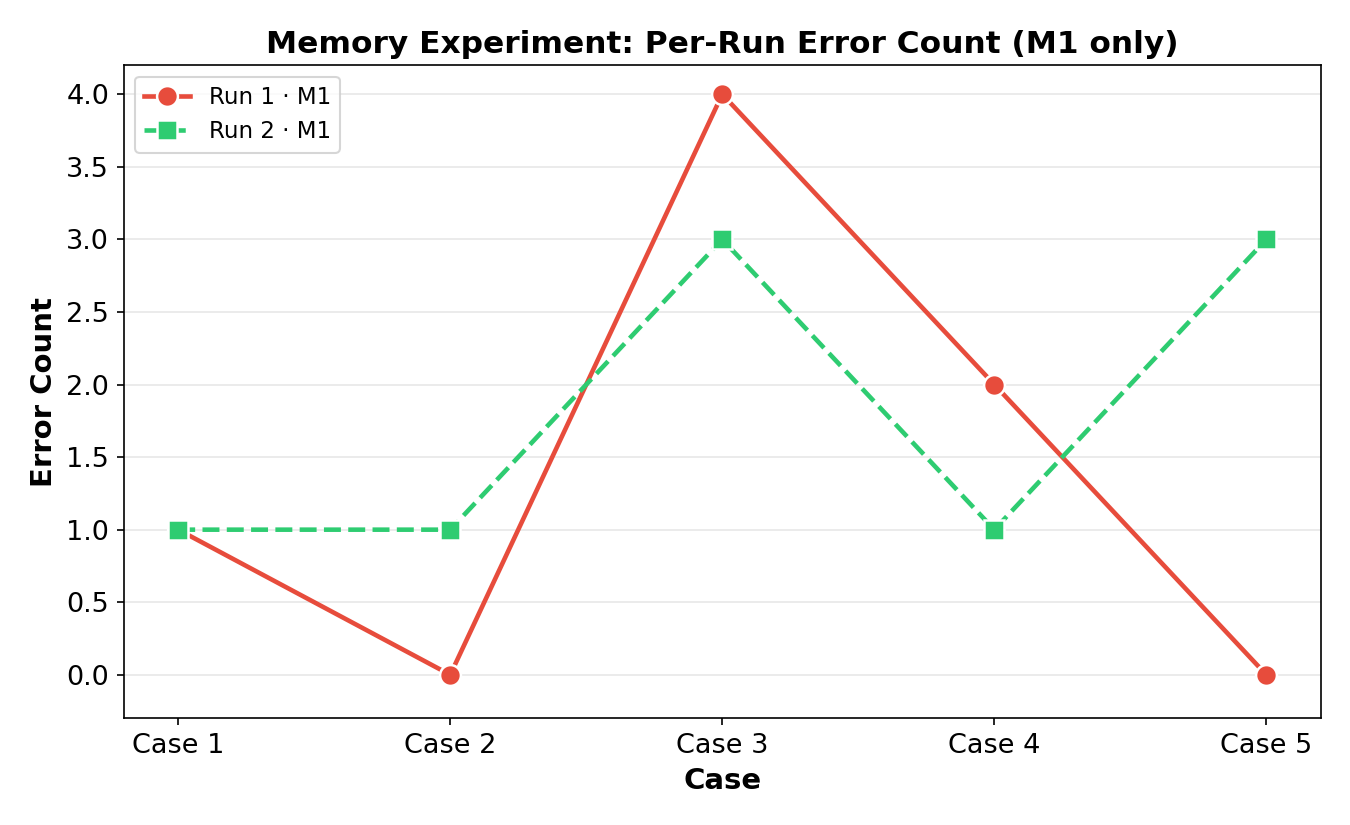
\includegraphics[width=0.80\textwidth]{memory_by_run.png}
  \caption{Memory 实验 M1 逐 run 错误计数}
\end{figure}

\begin{table}[htbp]
  \centering
  \caption{Memory M1 逐 run 结果}
  \begin{tabular}{@{}lcc@{}}
    \toprule
    Case & Run 1 & Run 2 \\
    \midrule
    C1 & 1 & 1 \\
    C2 & 0 & 1 \\
    C3 & 4 & 3 \\
    C4 & 2 & 1 \\
    C5 & 0 & 3 \\
    \midrule
    Sum & 7 & 9 \\
    \bottomrule
  \end{tabular}
\end{table}

\subsection{分错误类型}

\begin{figure}[htbp]
  \centering
  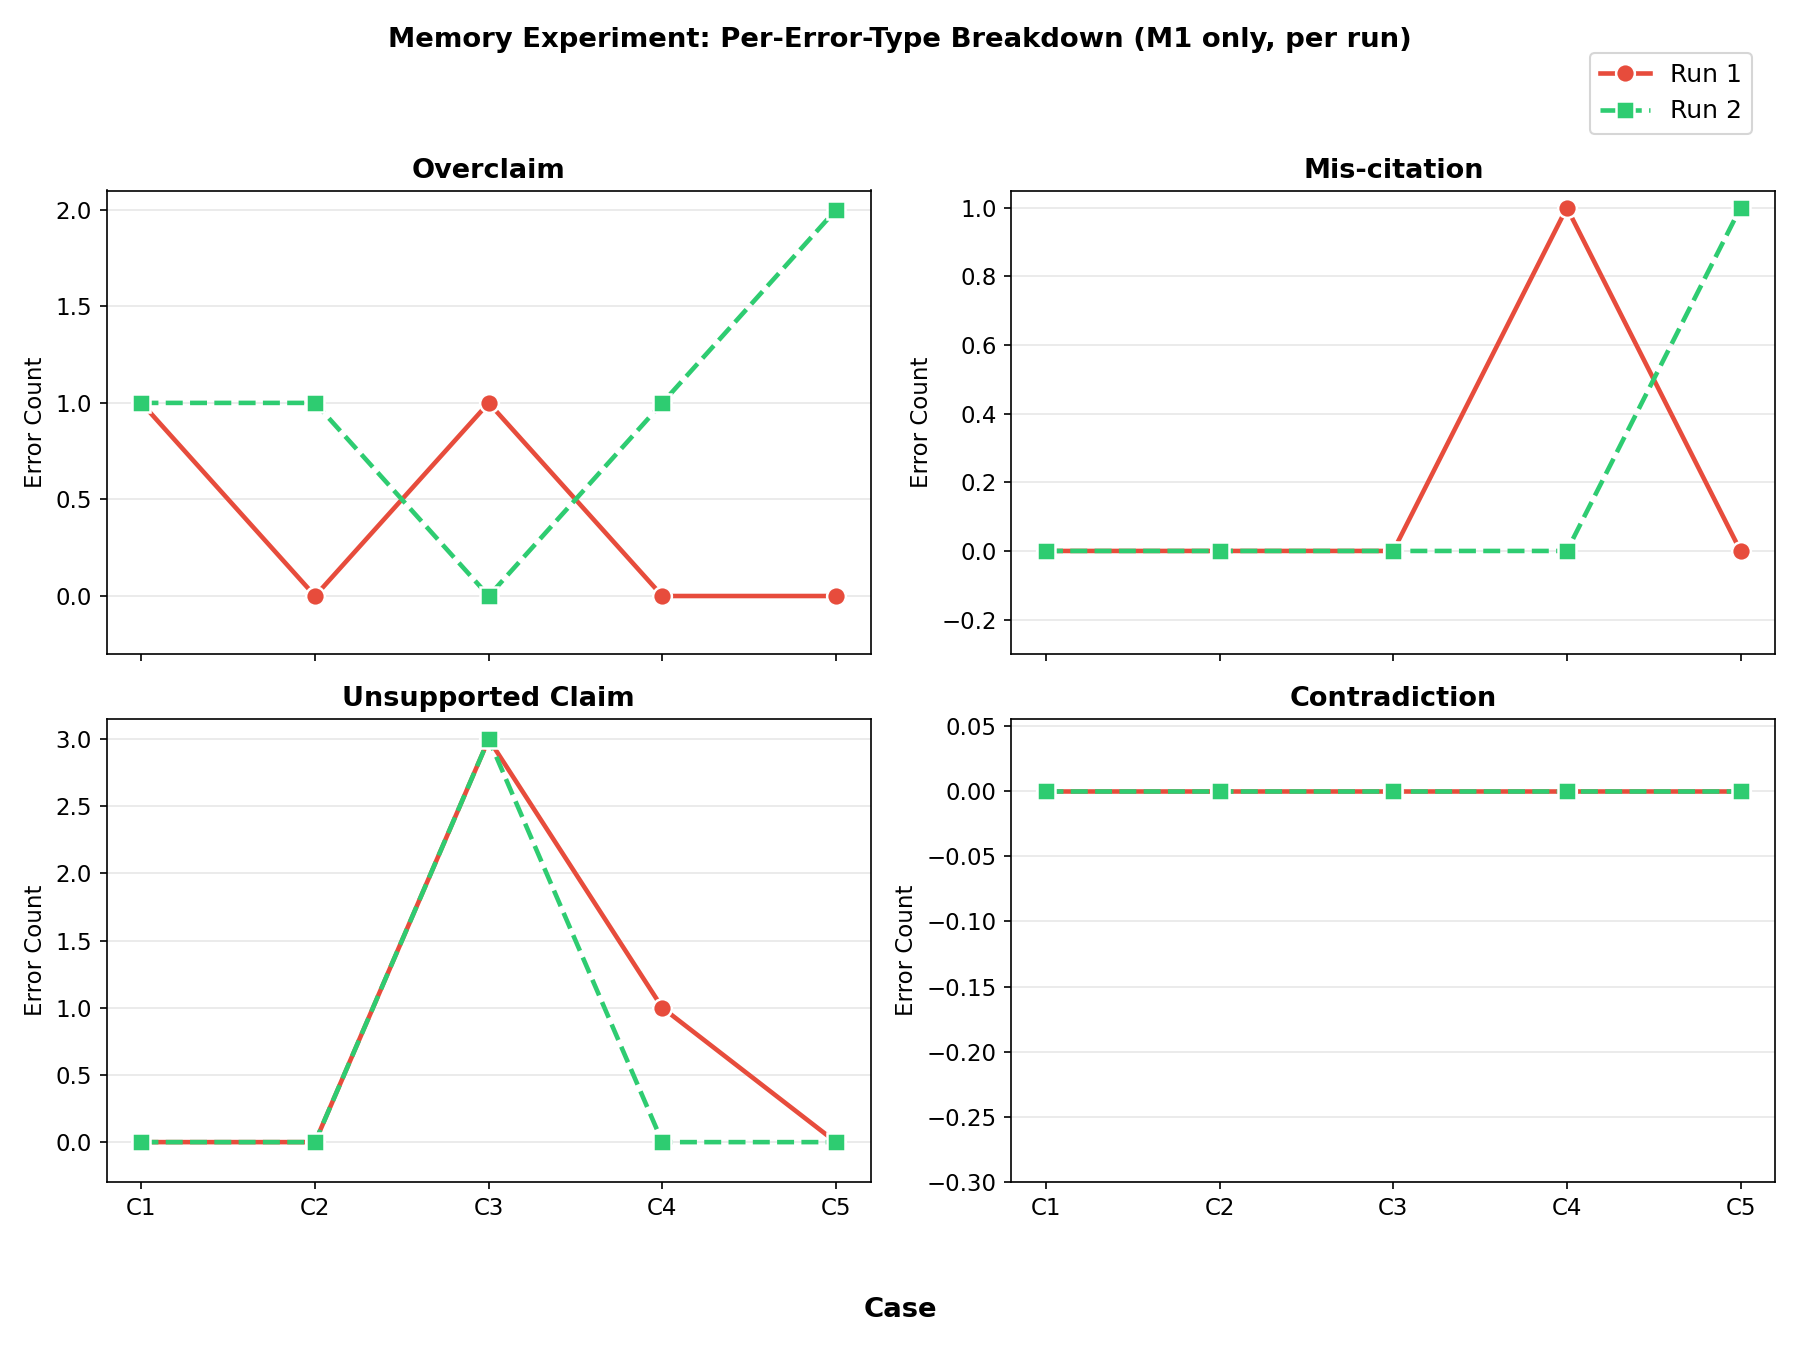
\includegraphics[width=0.95\textwidth]{memory_by_type.png}
  \caption{Memory 实验 M1 分错误类型}
\end{figure}

\begin{itemize}[nosep]
  \item \textbf{Overclaim}：Run1 C1=1, C3=1；Run2 C5=2 最多
  \item \textbf{Unsupported Claim}：\textbf{100\% 集中在 C3}，两 run 各 3 个
  \item \textbf{Contradiction}：\textbf{清零}——两 run 均无此类型
  \item \textbf{Mis-citation}：极少，Run1 C4=1, Run2 C5=1
\end{itemize}

\subsection{Memory vs Refchecker 对比}

\begin{figure}[htbp]
  \centering
  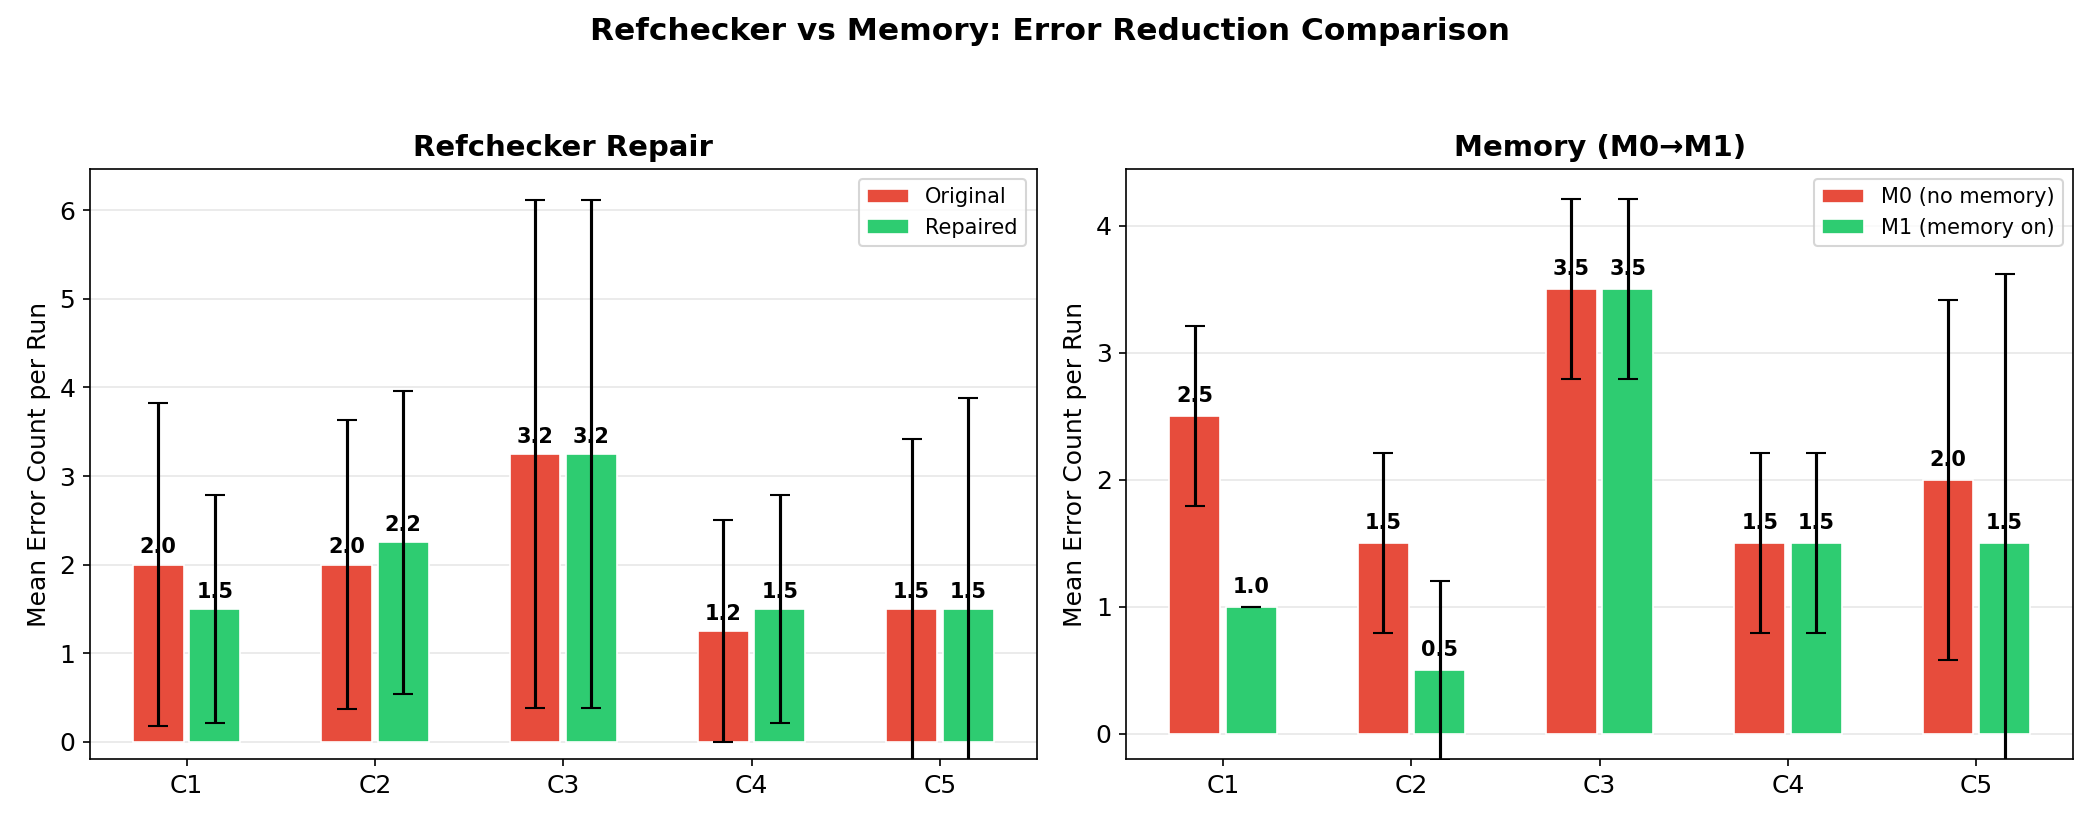
\includegraphics[width=0.90\textwidth]{memory_vs_refchecker.png}
  \caption{Refchecker Repair vs Memory 效果对比}
\end{figure}

\begin{table}[htbp]
  \centering
  \caption{Memory M0 vs M1 总览}
  \begin{tabular}{@{}lccc@{}}
    \toprule
    & M0 & M1 & 变化 \\
    \midrule
    Run1 & 11 & 7 & ↓ 36\% \\
    Run2 & 11 & 9 & ↓ 18\% \\
    \midrule
    Total & 22 & 16 & ↓ 27\% \\
    \bottomrule
  \end{tabular}
\end{table}

\textbf{Memory 减少错误总量 27\%，效果优于 refchecker repair（repair 总量不变）。}

% ===================================================================
\section{归因分析总结}
% ===================================================================

\begin{table}[htbp]
  \centering
  \caption{核心 Insight 总结}
  \begin{tabularx}{\textwidth}{@{}cXc@{}}
    \toprule
    \# & Insight & 支撑实验 \\
    \midrule
    1 & arxiv MCP 提升检索可验证性，不提升主题贴合度 & E1 \\
    2 & refchecker 做 Citation verification，不代替 Claim verification & E2 \\
    3 & repair 是错误类型漂移，不是错误消除 & E2 \\
    4 & 领域专业度越高，工具辅助越无效 & E2 + E3 \\
    5 & Memory 比 refchecker repair 更有效（↓27\% vs 0\%） & E3 \\
    6 & Memory 消除 Contradiction，但不解决 Unsupported Claim & E3 \\
    7 & C3（生化）是三个实验的共识 hard case & E1 + E2 + E3 \\
    8 & C1（主流 CS）从所有干预中获益最大 & E2 + E3 \\
    \bottomrule
  \end{tabularx}
\end{table}

\subsection{改进方向}

\begin{enumerate}[nosep]
  \item refchecker 之前加 source-grounded check：先让 Agent 逐句核对引用是否真的包含支撑信息
  \item 领域自适应策略：高专业度 case（如 C3）采用更保守的 claim 策略
  \item repair 改为迭代循环："改写 → 再核查 → 再改写"，目标消除而非转换
  \item Memory 写入来源扩展到 claim-level feedback，而不仅是 repair log
\end{enumerate}

% ===================================================================
\section{实验对比总表}
% ===================================================================

\begin{table}[htbp]
  \centering
  \caption{三个实验核心指标横向对比}
  \begin{tabular}{@{}lccc@{}}
    \toprule
    维度 & E1: arxiv MCP & E2: Refchecker & E3: Memory \\
    \midrule
    错误总量变化 & N/A & 40 → 40 (=) & 22 → 16 (↓27\%) \\
    C1 改善 & N/A & ↓ 0.7 & ↓ 最大 \\
    C3 改善 & N/A & = & = \\
    Contradiction & N/A & 不变 & \textbf{清零} \\
    核心机制 & 检索真实性提升 & 元数据验证 & 经验迁移 \\
    主要局限 & 不提升 relevance & 不验证语义支撑 & 领域知识鸿沟 \\
    \bottomrule
  \end{tabular}
\end{table}

% ===================================================================
\section{工程问题与解决方案}
% ===================================================================

本项目的难点不只在实验设计，也在于让一个多工具科研 Agent 评测真正可复现。实验过程中暴露出的很多问题都不是模型输出本身，而是工具链、网络、profile 隔离、引用材料组织方式和判定流水线之间的耦合。下面总结主要问题和对应处理方式。

\begin{table}[htbp]
  \centering
  \small
  \caption{运行环境与工具链问题}
  \begin{tabularx}{\textwidth}{@{}p{2.8cm}XX@{}}
    \toprule
    问题 & 现象 & 处理方式 \\
    \midrule
    arXiv 网络访问不稳定 &
    部分运行中 arXiv 域名被解析到异常地址，或 web search / web fetch 长时间超时。 &
    关闭 Clash Fake-IP 造成的虚拟网卡干扰；对 OpenClaw 运行显式设置 \texttt{HTTPS\_PROXY}、\texttt{HTTP\_PROXY} 和 \texttt{NO\_PROXY}，将 \texttt{arxiv.org} / \texttt{export.arxiv.org} 放入直连列表，保证 arXiv 直连、搜索服务走代理。 \\
    \addlinespace
    arxiv MCP 偶发 \texttt{-32000} 错误 &
    MCP server 单独握手正常，但 OpenClaw bundle-MCP 层有时无法稳定连接，且并行运行会放大该问题。 &
    将 arxiv MCP 作为预实验变量单独验证；主实验中固定使用安全 wrapper 和 Brave Search fallback。运行脚本强制 \texttt{JOBS=1}，避免多个 case 同时争用 MCP / web search。 \\
    \addlinespace
    多 profile 认证和工具配置漂移 &
    新建 OpenClaw profile 后出现 DeepSeek API key 缺失、Brave plugin 未安装、memory/session search 被意外启用等问题。 &
    为每个实验 profile 添加 profile audit；统一 web search provider 为 Brave；显式关闭与实验变量无关的 memory / session search；把模型、thinking level、workspace 路径写入 manifest。 \\
    \addlinespace
    workspace 污染 &
    不同 run 共用全局 workspace 时，下载论文、临时文件和 memory 写回可能互相影响。 &
    对预实验使用独立 profile / workspace；Memory MVP 只在 \texttt{M1\_memory\_on} 内按固定顺序共享 memory，其它条件隔离。所有 prompt、raw output、manifest、stderr、memory snapshot 都落到 run 目录。 \\
    \addlinespace
    并行运行导致不稳定 &
    \texttt{JOBS=2} 时 arXiv、web search、DeepSeek API 更容易 timeout，且 memory 顺序语义被破坏。 &
    所有 memory 相关主实验固定单线程顺序执行；失败时使用新的 \texttt{session\_key} suffix 重试，并保留 run log 判断哪些输出是有效证据。 \\
    \bottomrule
  \end{tabularx}
\end{table}

\begin{table}[htbp]
  \centering
  \small
  \caption{评测材料与判定流水线问题}
  \begin{tabularx}{\textwidth}{@{}p{2.8cm}XX@{}}
    \toprule
    问题 & 现象 & 处理方式 \\
    \midrule
    引用格式不可解析 &
    Agent 有时输出 \texttt{Abstract}、\texttt{第5页第3段} 或自由文本位置，无法稳定抽取 claim--citation pair。 &
    新增 \texttt{citation-standard} skill，要求 CPS 格式：文献 tag、section、段落/图/表等元素类型全部显式化；同时提供 \texttt{validate.py} 做格式检查。 \\
    \addlinespace
    refchecker 不等于 claim verification &
    refchecker 可以校对论文元数据，但不能判断"这篇论文是否真的支撑这个结论"。Repair 后常出现错误类型漂移，而不是错误消除。 &
    将 refchecker 定位为生成期辅助工具，而不是最终 evaluator；最终错误率另建 \texttt{evaluation/judge} 流水线，由 claim--citation pair + 论文局部证据片段交给 judge 独立判定。 \\
    \addlinespace
    P1/P2 文献包不完全重合 &
    同一个 case 中 P1 和 P2 可能把 \texttt{[D]}、\texttt{[E]} 指向不同论文；如果只在 \texttt{papers/} 中保存一份 \texttt{[D].pdf}，后续 judge 会读错证据。 &
    将展示与评测材料整理为可重建的 pass-specific 证据包；每个 pass 使用 pass-specific 文件名，例如 \texttt{P1\_[D]\_2405.17739.pdf} 与 \texttt{P2\_[D]\_2410.12944.md}。大文件证据包保留为本地缓存，仓库中保留 \texttt{evaluation/judge} 脚本、结构化输入和 source map。 \\
    \addlinespace
    LLM judge 成本和速度 &
    如果每条 claim 都让模型完整阅读 PDF，API 慢且成本高，长上下文也会降低判定稳定性。 &
    采用 local parser + locator snippet extraction + batched judge：先本地抽取 claim--citation pair 和定位片段，再每批 5--6 条送 DeepSeek 判断。PDF 缺失时使用 arXiv markdown 缓存，缺证据时标为 \texttt{NeedMoreContext} 或 \texttt{Unverifiable}。 \\
    \bottomrule
  \end{tabularx}
\end{table}

\subsection{对实验结论的影响}

这些工程问题直接影响评测可信度。首先，工具预实验必须和主实验解耦，否则 arxiv MCP 的连接问题会被误解释为 Agent 能力差异。其次，memory 实验必须按顺序执行，否则后续 case 的经验会提前污染前序 case。第三，最终 evaluator 不能依赖 Agent 自己的 refchecker repair log，因为这只是自我修复过程的一部分，而不是独立标注。最后，文献包必须按 pass 精确绑定，否则"引用与结论不一致"的错误率会混入材料组织错误。

因此，最终可复现材料不只包括报告输出，还包括 profile audit、run manifest、stderr、memory snapshot、claim--citation pair JSONL、judge batch prompt 和可重建的 paper source map。这些文件共同构成了本实验的复现边界。

\vspace{1em}
\begin{center}
\large\textbf{感谢阅读}
\end{center}

\end{document}
